% Copyright 2004 by Till Tantau <tantau@users.sourceforge.net>.
%
% In principle, this file can be redistributed and/or modified under
% the terms of the GNU Public License, version 2.
%
% However, this file is supposed to be a template to be modified
% for your own needs. For this reason, if you use this file as a
% template and not specifically distribute it as part of a another
% package/program, I grant the extra permission to freely copy and
% modify this file as you see fit and even to delete this copyright
% notice. 

\documentclass{beamer}
% Replace the \documentclass declaration above
% with the following two lines to typeset your 
% lecture notes as a handout:
%\documentclass{article}
%\usepackage{beamerarticle}

\usepackage{graphicx}
\usepackage[utf8]{inputenc}
 
\graphicspath{ {img/} }


% There are many different themes available for Beamer. A comprehensive
% list with examples is given here:
% http://deic.uab.es/~iblanes/beamer_gallery/index_by_theme.html
% You can uncomment the themes below if you would like to use a different
% one:
%\usetheme{AnnArbor}
%\usetheme{Antibes}
%\usetheme{Bergen}
%\usetheme{Berkeley}
%\usetheme{Berlin}
%\usetheme{Boadilla}
%\usetheme{boxes}
%\usetheme{CambridgeUS}
%\usetheme{Copenhagen}
%\usetheme{Darmstadt}
%\usetheme{default}
%\usetheme{Frankfurt}
%\usetheme{Goettingen}
%\usetheme{Hannover}
%\usetheme{Ilmenau}
%\usetheme{JuanLesPins}
%\usetheme{Luebeck}
%\usetheme{Madrid}
%\usetheme{Malmoe}
%\usetheme{Marburg}
%\usetheme{Montpellier}
%\usetheme{PaloAlto}
%\usetheme{Pittsburgh}
%\usetheme{Rochester}
%\usetheme{Singapore}
%\usetheme{Szeged}
\usetheme{Warsaw}

\title{Programming with NodeJS}

% A subtitle is optional and this may be deleted
\subtitle{Lesson 3: Time to get MEAN}

%\author{F.~Author\inst{1} \and S.~Another\inst{2}}
% - Give the names in the same order as the appear in the paper.
% - Use the \inst{?} command only if the authors have different
%   affiliation.

%\institute[Universities of Somewhere and Elsewhere] % (optional, but mostly needed)
%{
%  \inst{1}%
%  Department of Computer Science\\
%  University of Somewhere
%  \and
%  \inst{2}%
%  Department of Theoretical Philosophy\\
%  University of Elsewhere}
% - Use the \inst command only if there are several affiliations.
% - Keep it simple, no one is interested in your street address.

\date{Febuary 21st, 2017}
% - Either use conference name or its abbreviation.
% - Not really informative to the audience, more for people (including
%   yourself) who are reading the slides online

\subject{NodeJS Lessons}
% This is only inserted into the PDF information catalog. Can be left
% out. 

% If you have a file called "university-logo-filename.xxx", where xxx
% is a graphic format that can be processed by latex or pdflatex,
% resp., then you can add a logo as follows:

% \pgfdeclareimage[height=0.5cm]{university-logo}{university-logo-filename}
% \logo{\pgfuseimage{university-logo}}

% Delete this, if you do not want the table of contents to pop up at
% the beginning of each subsection:
%\AtBeginSubsection[]
%{
%  \begin{frame}<beamer>{Outline}
%    \tableofcontents[currentsection,currentsubsection]
%  \end{frame}
%}

% Let's get started
\begin{document}

\begin{frame}
  \titlepage
\end{frame}

%\begin{frame}{Outline}
%  \tableofcontents
%  % You might wish to add the option [pausesections]
%\end{frame}

% Section and subsections will appear in the presentation overview
% and table of contents.
\section{Introduction}

\begin{frame}{Summary of last week}
  Last week we:
  \pause
  \begin{itemize}
  \item We have learnt about callbacks and the NodeJS event loop\pause
  \item We have learnt about buffers\pause
  \item We have learnt about the Express framework\pause
  \item We have made a complex server using Express\pause
  \end{itemize}
  \pause
  Today, we are going to attempt a chat server using the MEAN stack.
\end{frame}

\section{Stacks and MEAN}

\begin{frame}{What is a web stack?}
A web stack is the suite of software someone uses to host their web service.\\
\pause
Common web stacks include:
\begin{itemize}
  \item LAMP \pause - Linux-Apache-MySQL-PHP \pause
  \item LEMP \pause - Linux-NGINX-MySQL-PHP \pause
  \item WISA \pause - Windows-IIS-msSQL-ASP.NET
\end{itemize}

\end{frame}

\begin{frame}{MEAN}

We are going to focus on the MEAN stack. The mean stack stands for:\pause
\begin{enumerate}
  \item M \pause - MongoDB \pause
  \item E \pause - ExpressJS \pause
  \item A \pause - AngularJS \pause
  \item N \pause - NodeJS
\end{enumerate}
\pause
Note, each of these are javascript-based. This is one of the major advantages of the MEAN stack, all software we will write using this stack will be in the same language.
\end{frame}

\begin{frame}{M - MongoDB}

MongoDB is a database management system (DBMS) written in C++ and javascript, which provides a nice way for us, as NodeJS developers, to store information.\\ \pause

MongoDB is classified as a NoSQL DBMS and is not similar to the SQL-family of DBMSs. Instead, MongoDB stores all its information as "loose" records called documents, wherein each of these documents follow a prewritten schema.\\ \pause

The format of these documents is in JSON. What this means is that we can simply pass a JSON to a MongoDB server and it will be able to store it, without having to change it to a certain format or something.

\end{frame}

\begin{frame}{E - ExpressJS}

As with last week, ExpressJS is a web framework for NodeJS allowing us to implement APIs and web services simply in high performance environments.\\ \pause

It has many potent features including powerful endpoint matching, templating and middleware utilities.\\ \pause

For more info, check out last weeks lesson.

\end{frame}

\begin{frame}{A - AngularJS}

AngularJS is a model-view-controller (MVC) framework for web frontend.\\ \pause

It provides all the functionality your browser needs to do cool stuff, which HTML is missing.\\ \pause

It injects itself into html:

\end{frame}

\begin{frame}{A - AngularJS}

Example

\end{frame}

\begin{frame}{N - NodeJS}

NodeJS is the backend that brings it all together. It lets express run on top of it and lets MongoDB communicate with the outside world.

\end{frame}

\begin{frame}{The MEAN stack altogether}

\begin{figure}[h]
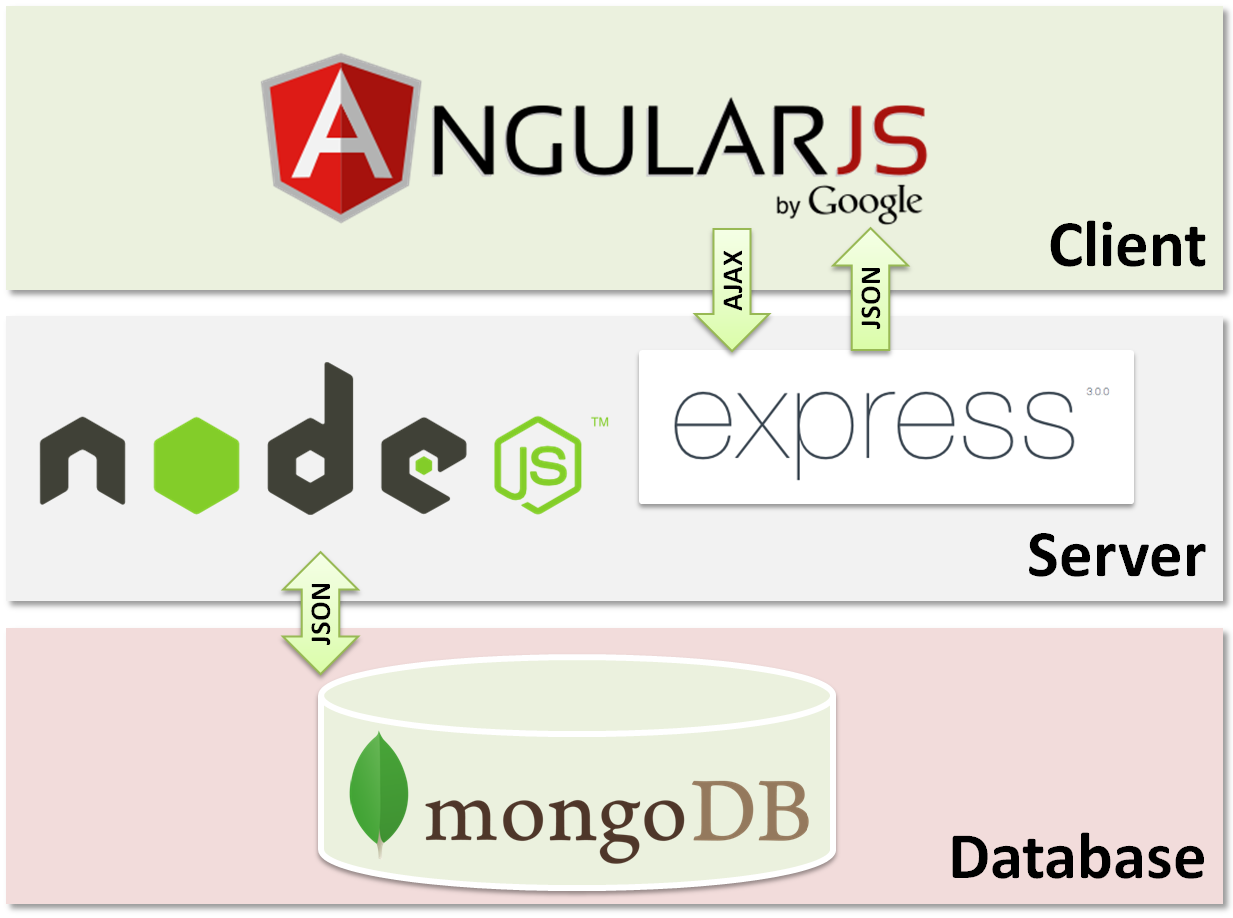
\includegraphics[width=0.8\textwidth]{mean-diagram}
\caption{Innocently stolen from: https://github.com/joaopsilva}
\end{figure}

\end{frame}
\section{Chat servers}
\begin{frame}{A quick note before the chat server}

There are two other libraries we will need to produce a chat server:
\begin{enumerate}
  \item Mongoose \pause - An interface that allows NodeJS to communicate with a MongoDB server \pause
  \item Socket.IO \pause - A web socket frontend and NPM which allows us to communicate with a browser in real time (as opposed to by sending HTTP requests)
\end{enumerate}

\end{frame}

\begin{frame}{Time to begin!}

Some handy links:
Socket.IO server side - https://github.com/socketio/socket.io\\
Socket.IO client side - https://github.com/socketio/socket.io-client\\
MongoDB download - https://www.mongodb.com/download-center\\
Bower install info - https://bower.io/ (or if you have npm: sudo npm install -g bower) \\
(All other dependencies are installed via NPM or bower: npm install --save mongoose express ejs socket.io \&\& bower install --save angular socket.io)

\end{frame}

\section{Summary}

\begin{frame}{That's all!}
  To summarise:
  \begin{itemize}
  \item We have learnt about each element in the MEAN stack
  \item We have learnt about socket IO and mongoose
  \item We have built our own chat box web app!
  \end{itemize}
\end{frame}

\begin{frame}{That's it folks!}
Source code plus lecture slides will be available online soon after the lesson.\\
If you are new to HackSocNotts, please join us on \textit{http://hacksocnotts.slack.com}.\\
If you have any questions, feel free to ask now or over slack.\\
Hope you enjoyed!
\end{frame}

\end{document}


